\documentclass{article}

\usepackage{graphicx}
\usepackage{tikz}
\usepackage{tikzsymbols}
\usetikzlibrary{calc,patterns,shapes.geometric}
\pagestyle{empty}
\usepackage[margin=0pt]{geometry}
\geometry{papersize={14in,12in}}

\def\centerarc[#1](#2)(#3:#4:#5){\draw[#1] ($(#2)+({#5*cos(#3)},{#5*sin(#3)})$) arc (#3:#4:#5);}

\begin{document}
	\begin{figure}
		\centering
		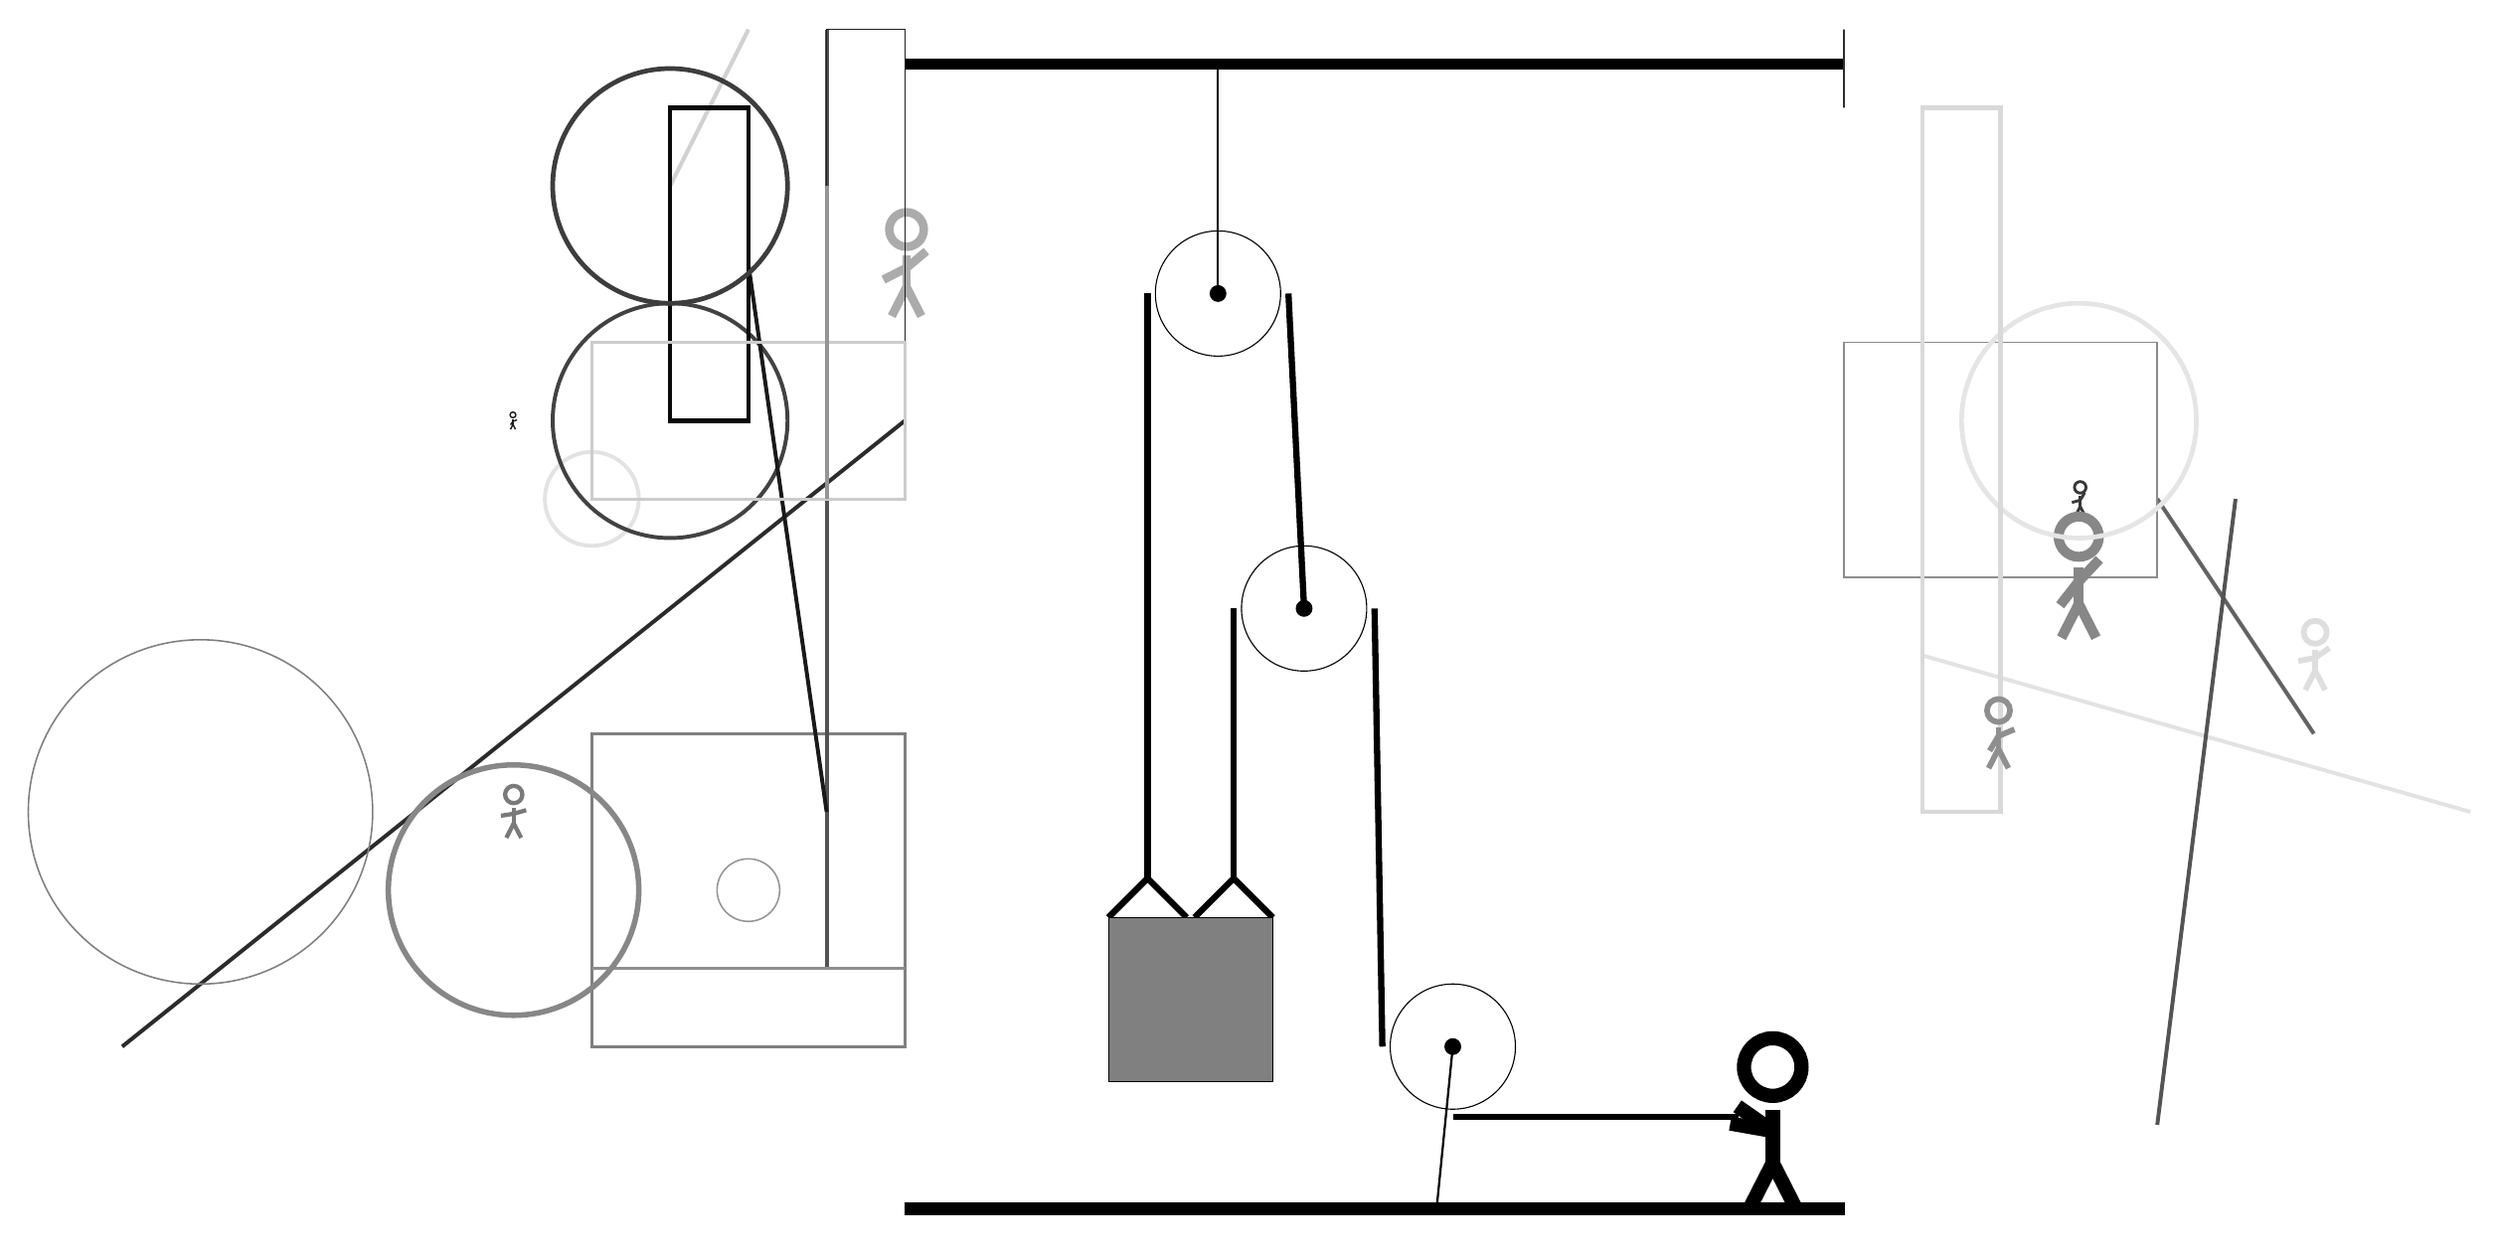
\begin{tikzpicture}
			%%%%% START %%%%%
			
			\draw[fill=black] (-2, 11.5) rectangle (10, 11.625);
			
			\draw (2, 8.625) circle (0.8);
			\draw[fill=black] (2, 8.625) circle (0.1);
			\draw[thick] (2, 8.625) -- (2, 11.5);
			
			\draw (3.1, 4.6) circle (0.8);
			\draw[fill=black] (3.1, 4.6) circle (0.1);
			
			\draw (5, -1) circle (0.8);
			\draw[fill=black] (5, -1) circle (0.1);
			\draw[thick] (5, -1) -- (4.8, -3);
			
			\draw[line width = 0.8mm]  (0.6, 0.65) -- (1.1, 1.15) -- (1.6, 0.65);
			\draw[line width = 0.8mm]  (1.7, 0.65) -- (2.2, 1.15) -- (2.7, 0.65);
			\draw[fill=black!50] (0.6, 0.65) rectangle (2.7, -1.45);
			
			\draw[line width=0.5mm, color=black!61](14, 6) -- (16, 3);
			
			\draw[line width=0.5mm, color=black!18](-4, 12) -- (-5, 10);
			\draw[line width=0.3mm, color=black!82] (10, 11) rectangle (10, 12);
			\draw[line width=0.5mm, color=black!11](11, 4) -- (18, 2);
			
			\node[line width=0.3mm, color=black!52] at (-7, 2) {\Strichmaxerl[3][9][16]};
			\draw[line width=0.2mm, color=black!45] (10, 5) rectangle (14, 8);
			
			\draw[line width=0.5mm, color=black!67](15, 6) -- (14, -2);
			\node[line width=0.3mm, color=black!13] at (16, 4) {\Strichmaxerl[4][11][35]};
			\draw[line width=0.4mm, color=black!50] (-2, 3) rectangle (-6, -1);
			
			\node[line width=0.7mm, color=black!78] at (13, 6) {\Strichmaxerl[2][16][59]};
			\node[line width=0.3mm, color=black!47] at (13, 5) {\Strichmaxerl[7][52][47]};
			\draw[line width=0.5mm, color=black!68](-3, 0) -- (-3, 12);
			\draw [line width=0.5mm, color=black!11](-6, 6) circle (0.6);
			
			\draw[line width=0.5mm, color=black!83](-2, 7) -- (-12, -1);
			\draw [line width=0.2mm, color=black!41](-4, 1) circle (0.4);
			\node[line width=0.4mm, color=black!88] at (-7, 7) {\Strichmaxerl[1][55][19]};
			
			\draw [line width=0.6mm, color=black!10](13, 7) circle (1.5);
			\draw [line width=0.2mm, color=black!50](-11, 2) circle (2.2);
			\draw [line width=0.5mm, color=black!74](-5, 7) circle (1.5);
			\node[line width=0.2mm, color=black!33] at (-2, 9) {\Strichmaxerl[6][27][40]};
			\draw[line width=0.6mm, color=black!15] (12, 2) rectangle (11, 11);
			\draw[line width=0.5mm, color=black!90](-3, 2) -- (-4, 9);
			\draw[line width=0.4mm, color=black!44] (-2, 0) rectangle (-6, 0);
			\node[line width=0.5mm, color=black!44] at (12, 3) {\Strichmaxerl[4][59][23]};
			\draw[line width=0.6mm, color=black!96] (-4, 11) rectangle (-5, 7);
			
			\draw[line width=0.2mm, color=black!87] (-3, 12) rectangle (-2, 6);
			\draw[line width=0.4mm, color=black!20] (-2, 6) rectangle (-6, 8);
			\draw [line width=0.6mm, color=black!76](-5, 10) circle (1.5);
			
			\draw [line width=0.7mm, color=black!47](-7, 1) circle (1.6);
			\draw[line width=0.5mm, color=black!42] (-3, 10) rectangle (-3, 6);
			
			\draw[line width = 0.8mm] (1.1, 8.625) -- (1.1, 1.15);
			\centerarc[line width = 0.8mm](2, 8.625)(0:180:0.9);
			\draw[line width = 0.8mm] (2.9, 8.625) -- (3.1, 4.6);
			\draw[line width = 0.8mm] (2.2, 4.6) -- (2.2, 1.15);
			\centerarc[line width = 0.8mm](3.1, 4.6)(0:180:0.9);
			\draw[line width = 0.8mm] (4.0, 4.6) -- (4.1, -1);
			\centerarc[line width = 0.8mm](5, -1)(180:270:0.9);
			\draw[line width = 0.8mm] (5, -1.9) -- (8.65, -1.9);
			
			\node at (9, -2) {\Strichmaxerl[10][-35][170]};
			
			\draw[fill=black] (-2, -3) rectangle (10, -3.15);
			
			%%%%% END %%%%%
		\end{tikzpicture}
	\end{figure}	
\end{document}